\documentclass{beamer}

%\usepackage[table]{xcolor}
\mode<presentation> {
  \usetheme{Boadilla}
%  \usetheme{Pittsburgh}
%\usefonttheme[2]{sans}
\renewcommand{\familydefault}{cmss}
%\usepackage{lmodern}
%\usepackage[T1]{fontenc}
%\usepackage{palatino}
%\usepackage{cmbright}
  \setbeamercovered{transparent}
\useinnertheme{rectangles}
}
%\usepackage{normalem}{ulem}
%\usepackage{colortbl, textcomp}
\setbeamercolor{normal text}{fg = black}
\setbeamercolor{structure}{fg = blue}
\definecolor{trial}{cmyk}{1,0,0, 0}
\definecolor{trial2}{cmyk}{0.00,0,1, 0}
\definecolor{darkgreen}{rgb}{0,.4, 0.1}
\definecolor{mygray}{gray}{0.8}
\definecolor{myblack}{rgb}{0, 0, 0}
\usepackage{array}
\beamertemplatesolidbackgroundcolor{white}  \setbeamercolor{alerted
text}{fg=red}

\setbeamertemplate{caption}[numbered]\newcounter{mylastframe}

\usepackage{color}
\usepackage{tikz}
\usetikzlibrary{arrows}
\usepackage{colortbl}
\usepackage{graphicx}
\usepackage{epsfig}

%\usepackage[usenames, dvipsnames]{color}
%\setbeamertemplate{caption}[numbered]\newcounter{mylastframe}c
%\newcolumntype{Y}{\columncolor[cmyk]{0, 0, 1, 0}\raggedright}
%\newcolumntype{C}{\columncolor[cmyk]{1, 0, 0, 0}\raggedright}
%\newcolumntype{G}{\columncolor[rgb]{0, 1, 0}\raggedright}
%\newcolumntype{R}{\columncolor[rgb]{1, 0, 0}\raggedright}

%\begin{beamerboxesrounded}[upper=uppercol,lower=lowercol,shadow=true]{Block}
%$A = B$.
%\end{beamerboxesrounded}}
\renewcommand{\familydefault}{cmss}
%\usepackage[all]{xy}

\usepackage{tikz}
\usepackage{lipsum}

 \newenvironment{changemargin}[3]{%
 \begin{list}{}{%
 \setlength{\topsep}{0pt}%
 \setlength{\leftmargin}{#1}%
 \setlength{\rightmargin}{#2}%
 \setlength{\topmargin}{#3}%
 \setlength{\listparindent}{\parindent}%
 \setlength{\itemindent}{\parindent}%
 \setlength{\parsep}{\parskip}%
 }%
\item[]}{\end{list}}
\usetikzlibrary{arrows}
%\usepackage{palatino}
%\usepackage{eulervm}
\usecolortheme{lily}

\newtheorem{com}{Comment}
\newtheorem{lem} {Lemma}
\newtheorem{prop}{Proposition}
\newtheorem{thm}{Theorem}
\newtheorem{defn}{Definition}
\newtheorem{cor}{Corollary}
\newtheorem{obs}{Observation}
 \numberwithin{equation}{section}


\title[PLSC 43401] % (optional, nur bei langen Titeln nötig)
{Mathematical Foundations of Political Methodology}

\author{Robert Gulotty}
\institute[University of Chicago]{Associate Professor\\Department of Political Science \\  University of Chicago}
\vspace{0.3in}
\date{August 28th, 2017}

\setbeamertemplate{navigation symbols}{}

\begin{document}

\begin{frame}
\titlepage
\end{frame}



\begin{frame}

\begin{itemize}
\item \textcolor{myblack}{Vectors}
\item \textcolor{myblack}{Matrix}
\item \textcolor{myblack}{Matrix Algebra}
\item \textcolor{myblack}{Matrix Inversion}
\end{itemize}

\end{frame}



\begin{frame}

\begin{itemize}
\item \textcolor{myblack}{Vectors}
\item \textcolor{mygray}{Matrix}
\item \textcolor{mygray}{Matrix Algebra}
\item \textcolor{mygray}{Matrix Inversion}
\end{itemize}

\end{frame}



\begin{frame}
\frametitle{Points and Vectors} 

\begin{defn} 
A point $\boldsymbol{x} \in R^{n}$ is an ordered n-tuple, $(x_{1}, x_{2}, \hdots, x_{n})$.  The vector $\boldsymbol{x} \in R^{n}$ is the arrow pointing from the origin $(0, 0, \hdots, 0)$ to $\boldsymbol{x}$. \end{defn} \pause

Some Examples: \pause
\begin{itemize}
\item[-] (Latitude, Longitude, Elevation)
\item[-] (1, 2, 3)
\item[-] (0, 1, 0)
\end{itemize}

\end{frame}



\begin{frame}
\frametitle{Points and Vectors}

\ \\Now, let's see a vector in a 2 dimensional space.

\begin{center}
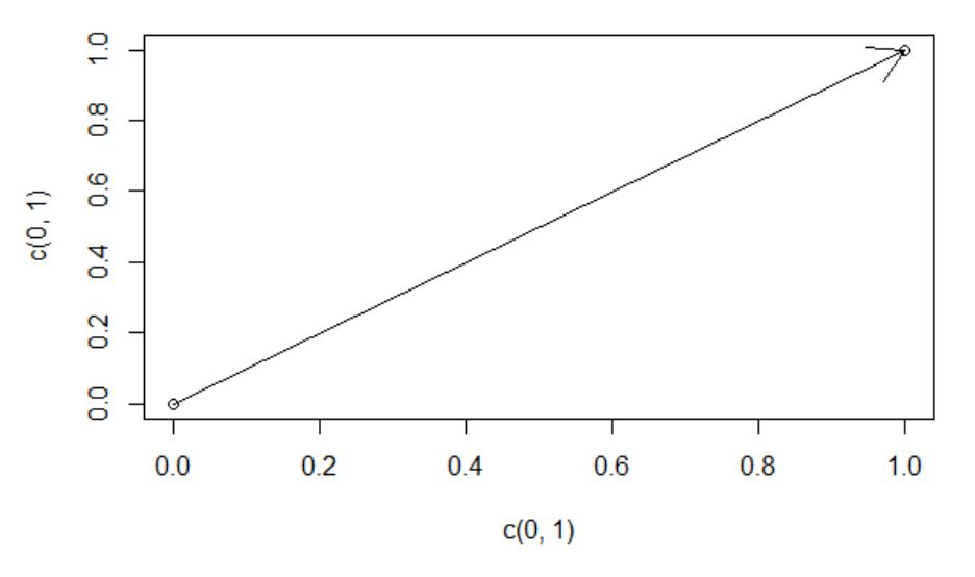
\includegraphics[scale = 0.5]{plsc43401_lec6_pic_1.eps}
\end{center}

\end{frame}



\begin{frame}
\frametitle{Points and Vectors}

\ \\Now, let's see a vector in a 3 dimensional space.

\begin{center}
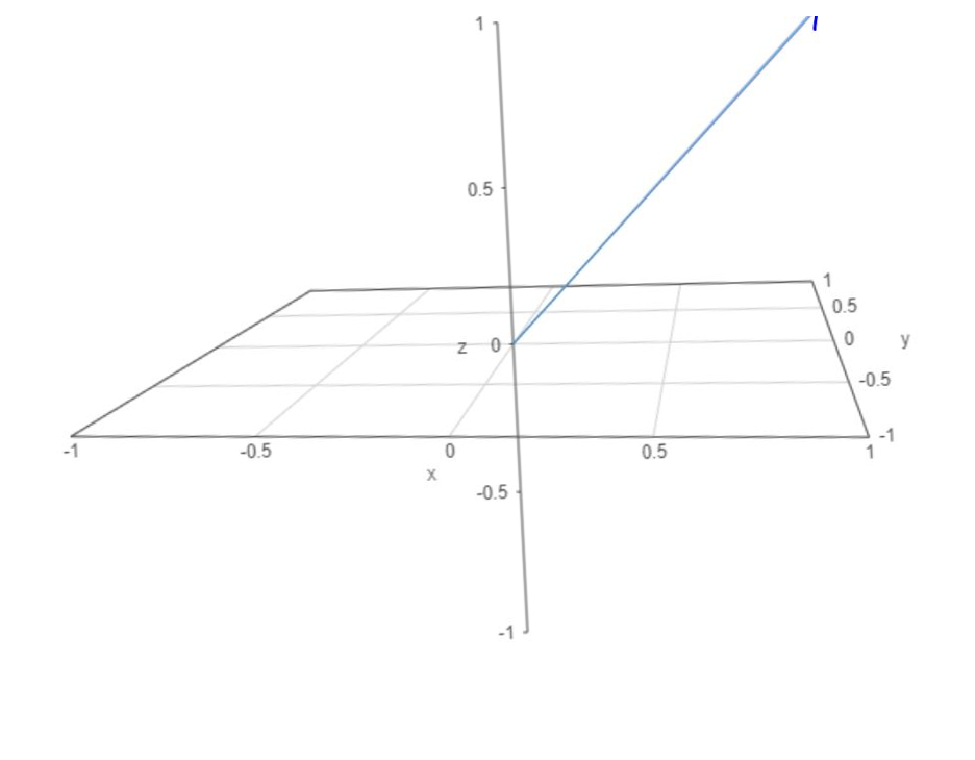
\includegraphics[scale = 0.5]{plsc43401_lec6_pic_2.eps}
\end{center}

\end{frame}



\begin{frame}
\frametitle{Arithmetic with Vectors} 

\begin{defn} Suppose $\boldsymbol{u}$ and $\boldsymbol{v}$ are vectors $ \boldsymbol{u}, \boldsymbol{v} \in R^{n}$, \\

\begin{eqnarray}
\boldsymbol{u} & = & (u_{1}, u_{2}, u_{3}, \hdots, u_{n} ) \nonumber \\
\boldsymbol{v} & = & (v_{1}, v_{2}, v_{3}, \hdots, v_{n} ) \nonumber 
\end{eqnarray}
We will say $\boldsymbol{u} = \boldsymbol{v}$ if $u_{1} = v_{1}, u_{2} = v_{2}, \hdots, u_{n} = v_{n} $\\ \pause

Define the sum of $\boldsymbol{u} + \boldsymbol{v}$ as 
\begin{eqnarray}
\boldsymbol{u} + \boldsymbol{v} & = & (u_{1} + v_{1}, u_{2} + v_{2}, u_{3} + v_{3}, \hdots, u_{n} + v_{n} ) \nonumber 
\end{eqnarray} \pause

Suppose $k \in R$.  We will call $k$ a scalar.\\

Define $k \boldsymbol{u}$ as the scalar product

$$k \boldsymbol{u} = (k u_{1}, k u_{2}, \hdots, k u_{n} )$$ 

\end{defn}

\end{frame}



\begin{frame}
\frametitle{Examples} 

Suppose:
\begin{eqnarray}
\boldsymbol{u} & = & (1, 2, 3, 4, 5) \nonumber \\
\boldsymbol{v} & = & (1, 1, 1, 1, 1) \nonumber \\
k & = & 2 \nonumber 
\end{eqnarray} \pause

Then, 
\begin{eqnarray}
\boldsymbol{u}  + \boldsymbol{v} & = & (1 + 1, 2 + 1, 3+ 1, 4 + 1, 5+ 1)  = (2, 3, 4, 5, 6)\nonumber \\ \pause
k \boldsymbol{u} & = & (2 \times 1, 2 \times 2, 2 \times 3, 2 \times 4, 2 \times 5) = (2, 4, 6, 8, 10) \nonumber \\ \pause
k \boldsymbol{v} & = & (2 \times 1,2 \times 1,2 \times 1,2 \times 1,2 \times 1) = (2, 2, 2, 2, 2) \nonumber 
\end{eqnarray}

\end{frame}



\begin{frame}
\frametitle{Euclidean Norm of a Vector}

\ \\Now, a question will be: how do we measure the length of a vector. \pause

\ \\One way is to use Euclidean norm to measure the length of a vector \pause

\begin{defn}
On an n-dimensional Euclidean space $R^{n}$, the Euclidean norm of vector, $x = (x_{1}, x_{2}, ..., x_{n})$, is defined by the formula

$$ ||x||_{2} :={\sqrt {x_{1}^{2} + \cdots + x_{n}^{2}}}. $$
\end{defn} \pause

\ \\An example. What's the Euclidean norm of $x = (1, 3, 5)$?

\ \\Its Euclidean norm equals to:
$$ \sqrt[]{1^{2} + 3^{2} + 5^{2}} = \sqrt[]{35}$$.

\end{frame}



\begin{frame}

\begin{itemize}
\item \textcolor{mygray}{Vectors}
\item \textcolor{myblack}{Matrix}
\item \textcolor{mygray}{Matrix Algebra}
\item \textcolor{mygray}{Matrix Inversion}
\end{itemize}

\end{frame}



\begin{frame}
\frametitle{Matrices}

\ \\Now, let's see some examples for using matrices. \pause

\ \\The first example is the following system of equations: \pause

\begin{eqnarray}
2x + 2y + 3z &=& 1 \nonumber \\ 
3x + 5y + 7z &=& 2 \nonumber \\ 
5x + 8y + 3z &=& 3 \nonumber
\end{eqnarray} \pause

\ \\The coefficient of unknowns can be written compactly as matrices:

$ \begin{bmatrix}
    2 & 2 & 3 \\
    3 & 5 & 7 \\
    5 & 8 & 3
\end{bmatrix} $

\end{frame}



\begin{frame}
\frametitle{Matrices}

\ \\A second example of matrix is the data set.

\begin{center}
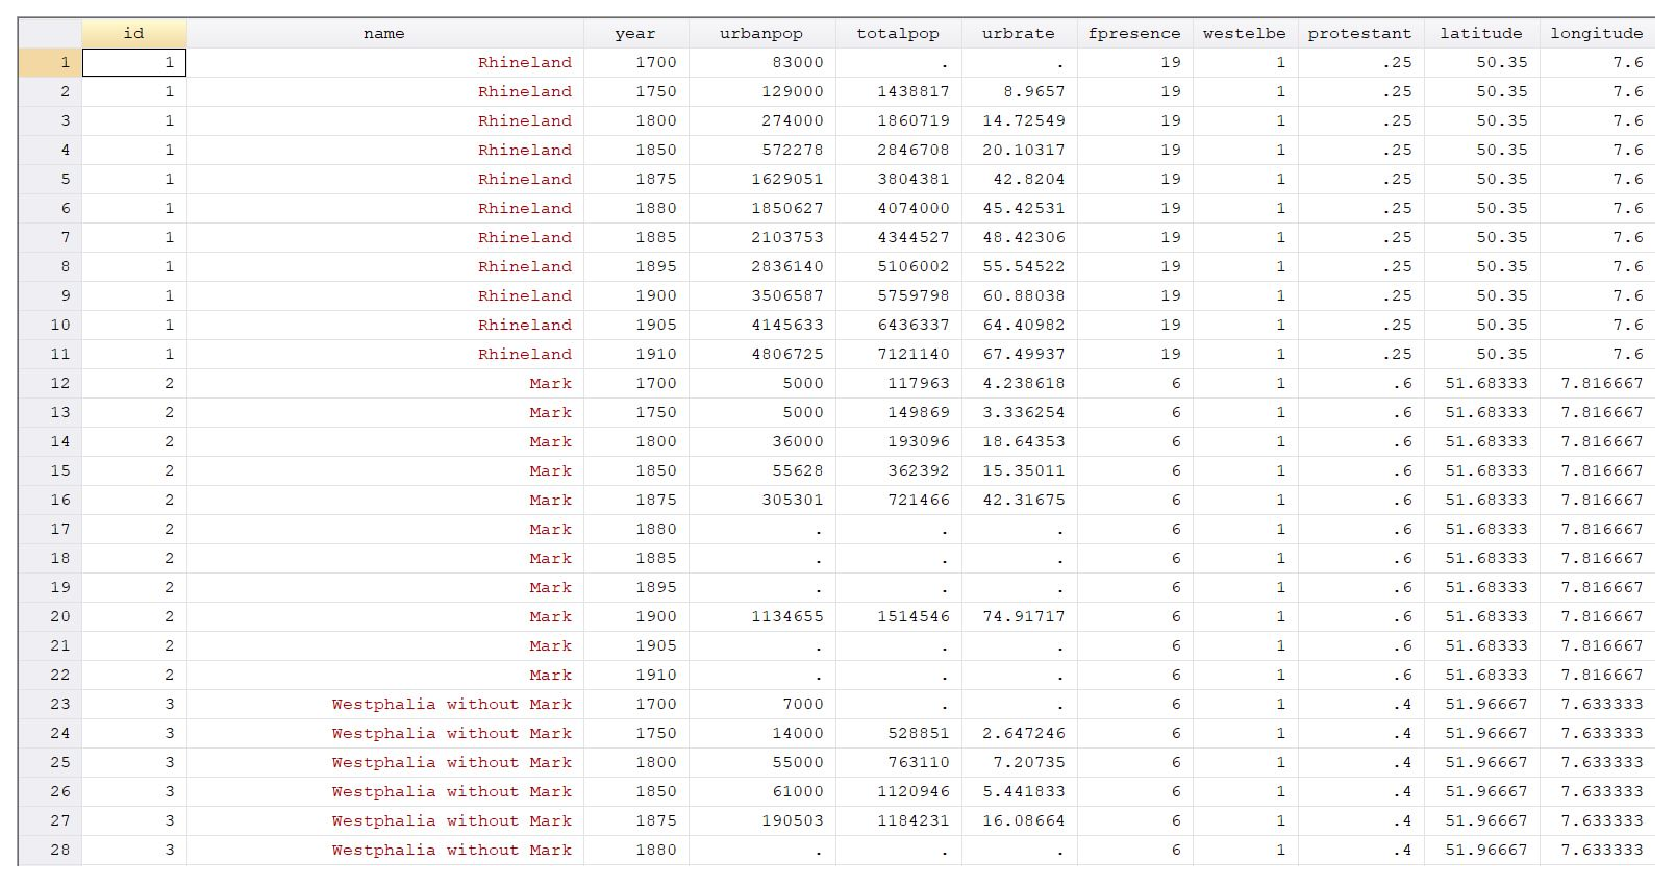
\includegraphics[scale = 0.36]{plsc43401_lec6_pic_3.eps}
\end{center}

\end{frame}



\begin{frame}
\frametitle{Matrices}

\begin{defn}
A Matrix is a rectangular array of numbers


\begin{eqnarray}
\boldsymbol{A} & = &  
\begin{pmatrix}
a_{11} & a_{12} & \hdots & a_{1n} \\
a_{21} & a_{22} & \hdots & a_{2n} \\
\vdots & \vdots & \ddots & \vdots \\
a_{m1} & a_{m2} & \hdots & a_{mn} \\
\end{pmatrix} 
\nonumber 
\end{eqnarray}
If $\boldsymbol{A}$ has $m$ rows $n$ columns (Roman Catholic; Rum \& Cake) we will say that $\boldsymbol{A}$ is an $m \times n$ matrix.  \\
Suppose $\boldsymbol{X}$ and $\boldsymbol{Y}$ are $m \times n$ matrices.  Then $\boldsymbol{X} = \boldsymbol{Y}$ if 
$x_{ij} = y_{ij}$ for all $i$ and $j$ 

\end{defn}
\end{frame}



\begin{frame}
\frametitle{Simple Examples} 

\begin{eqnarray} 
\boldsymbol{I} & = & \begin{pmatrix} 
1 & 0 & 0 & \hdots & 0 \\
0 & 1 & 0 & \hdots & 0 \\
0 & 0 & 1 & \hdots & 0 \\
\vdots & \vdots & \vdots & \ddots & \vdots \\
0 & 0 & 0 & \hdots & 1 \\
\end{pmatrix} 
\nonumber 
\end{eqnarray}
If $\boldsymbol{I}$ is an $n \times n$ matrix we will call an identity matrix.  

\end{frame}



\begin{frame}
\frametitle{Simple Examples} 

\begin{eqnarray}
\boldsymbol{X} & = & \begin{pmatrix} 
1 & 2 & 3 \\
2 & 1 & 4 \\
\end{pmatrix} 
\nonumber 
\end{eqnarray}
$\boldsymbol{X}$ is an $2 \times 3$ matrix

\end{frame}



\begin{frame}

\begin{itemize}
\item \textcolor{mygray}{Vectors}
\item \textcolor{mygray}{Matrix}
\item \textcolor{myblack}{Matrix Algebra}
\item \textcolor{mygray}{Matrix Inversion}
\end{itemize}

\end{frame}



\begin{frame}
\frametitle{Matrix Algebra}
\begin{defn} Suppose $\boldsymbol{X}$ and $\boldsymbol{Y} $ are $m \times n$ matrices.  Then define 
\begin{eqnarray} 
\boldsymbol{X} + \boldsymbol{Y} & = & \begin{pmatrix} 
x_{11} & x_{12} & \hdots & x_{1n} \\
x_{21} & x_{22} & \hdots & x_{2n} \\
\vdots & \vdots & \ddots & \vdots \\
x_{m1} & x_{m2} & \hdots & x_{mn} \\
\end{pmatrix} + 
\begin{pmatrix} 
y_{11} & y_{12} & \hdots & y_{1n} \\
y_{21} & y_{22} & \hdots & y_{2n} \\
\vdots & \vdots & \ddots & \vdots \\
y_{m1} & y_{m2} & \hdots & y_{mn} \\
\end{pmatrix}
\nonumber \\
& = & \begin{pmatrix} 
x_{11} + y_{11} & x_{12} + y_{12} & \hdots & x_{1n} + y_{1n} \\
x_{21} + y_{21} & x_{22} + y_{22} & \hdots & x_{2n} + y_{2n} \\
\vdots & \vdots & \ddots & \vdots\\
x_{m1} + y_{m1} & x_{m2} + y_{m2} & \hdots & x_{mn} + y_{mn} \\
\end{pmatrix} 
\nonumber 
\end{eqnarray}

\end{defn}

\end{frame}



\begin{frame}
\frametitle{Matrix Algebra} 
\begin{defn}
Suppose $\boldsymbol{X}$ is an $m \times n$ matrix and $k \in R$.  Then, 
\begin{eqnarray}
k \boldsymbol{X} & =&  \begin{pmatrix} 
k x_{11} & k x_{12} & \hdots &  k x_{1n} \\
k x_{21} & k x_{22} & \hdots & k x_{2n} \\
\vdots & \vdots & \ddots & \vdots \\
k x_{m1} & k x_{m2} & \hdots & k x_{mn} \\
\end{pmatrix}
\nonumber 
\end{eqnarray}

\end{defn}

\end{frame}



\begin{frame}
\frametitle{Matrix Transpose} 

We will use matrix transpose to flip the dimensionality of a matrix \pause \\

\begin{eqnarray}
\boldsymbol{X} & = & \begin{pmatrix} 
 \alert<3>{x_{11}} & \alert<3>{x_{12}} & \hdots & \alert<3>{x_{1n}} \\
\alert<4>{x_{21}} & \alert<4>{x_{22}} & \alert<4>{\hdots} & \alert<4>{x_{2n}} \\
\vdots & \vdots & \ddots & \vdots \\}
\alert<6>{x_{m1}} & \alert<6>{x_{m2}} & \hdots & \alert<6>{x_{mn} } \\
\end{pmatrix}}  \nonumber  \\
\boldsymbol{X}^{'} &  = &  \begin{pmatrix} 
\alert<3>{x_{11}}} &  \invisible<1-3>{ \alert<4>{x_{21} } }& \invisible<1-4>{\hdots} & \invisible<1-5>{\alert{x_{m1} } \\
\alert<3>{x_{12}}} & \invisible<1-3>{\alert<4>{x_{22} } }& \invisible<1-4>{\hdots} & \invisible<1-5>{\alert{x_{m2} } \\
\vdots }&\invisible<1-3>{ \vdots} & \invisible<1-4>{\ddot} & \invisible<1-5>{\vdots} \\
\alert<3>{x_{1n} }} & \invisible<1-3>{\alert<4>{x_{2n}}} & \invisible<1-4>{\hdots} & \invisible<1-5>{\alert{x_{mn} }\\
\end{pmatrix} }
\nonumber 
\end{eqnarray}


\invisible<1-6>{If $\boldsymbol{X}$ is an $m \times n$ then $\boldsymbol{X}^{'} $ is $n \times m$.}   \\
\invisible<1-7>{If $\boldsymbol{X} = \boldsymbol{X}^{'}$ then we say $\boldsymbol{X}$ is symmetric. }  

\pause\pause \pause \pause \pause \pause 
\end{frame}



\begin{frame}
\frametitle{Matrix Transpose}

Example 1:  $\boldsymbol{X} = \begin{pmatrix} 4 & 1 & 2 \\1 & 2  & 3 \\ \end{pmatrix} $ then 
$\boldsymbol{X}^{'} = \begin{pmatrix} 4 & 1 \\ 1 & 2 \\ 2 & 3 \\ \end{pmatrix} $ \\
\end{frame}



\begin{frame}
\frametitle{Matrix Multiplication}

How do we multiply matrices? \pause \\
Because we want to use matrix multiplication to solve equations we won't use an intuitive definition \pause \\

Suppose we have two matrices \pause  \\
$\boldsymbol{X} = \begin{pmatrix} 1 & 1 \\ 1& 1 \\ \end{pmatrix} $, $\boldsymbol{Y} = \begin{pmatrix} 1 & 2 \\ 3 & 4 \\ \end{pmatrix} $ \pause 

We will create a new matrix $\boldsymbol{A}$ by matrix multiplication: \pause 
\begin{eqnarray} 
\boldsymbol{A} & = & \boldsymbol{X} \boldsymbol{Y} \nonumber  \pause \\
				& = & \begin{pmatrix} \alert<8-9>{1} & \alert<8-9>{1} \\ \alert<10-11>{1}& \alert<10-11>{1}\\ \end{pmatrix} \begin{pmatrix} \alert<8,10>{1} & \alert<9,11>{2} \\ \alert<8,10>{3} & \alert<9,11>{4} \\ \end{pmatrix}
\nonumber  \pause \\
     					\invisible<1-7>{& = & \begin{pmatrix} }
							\invisible<1-7>{1 \times 1 + 1 \times 3}  & \invisible<1-8>{1 \times 2 + 1 \times 4}  \\
							\invisible<1-9>{1 \times 1  + 1\times 3}  & \invisible<1-10>{1 \times 2 + 1 \times 4 }  \\
							\invisible<1-7>{\end{pmatrix}} \nonumber \\
					\invisible<1-11>{& = & \begin{pmatrix} 
							4 & 6 \\
							4 & 6 \\
							\end{pmatrix}		}
							\nonumber 
\end{eqnarray}							
\pause \pause \pause\pause  												
\end{frame}



\begin{frame}
\frametitle{Matrix Multiplication}

\begin{defn} Suppose $\boldsymbol{X}$ is an $m \times n$ matrix and $\boldsymbol{Y}$ is an $n \times k$ matrix.  Then define the matrix $\boldsymbol{A}$ an $m \times k$ matrix that obtains from multiplying $\boldsymbol{X}$ and $\boldsymbol{Y}$ as, 
\small
\begin{eqnarray}
\boldsymbol{A} & = & \boldsymbol{X} \boldsymbol{Y} \nonumber \\
						& = & \begin{pmatrix} 
								x_{11} & x_{12} & \hdots & x_{1n} \\
								x_{21} & x_{22} & \hdots & x_{2n} \\
								\vdots & \vdots & \ddots & \vdots \\
								x_{m1} & x_{m2} & \hdots & x_{mn} \\
								\end{pmatrix} 
								\begin{pmatrix} 
								y_{11} & y_{12} & \hdots & y_{1k} \\
								y_{21} & y_{22} & \hdots & y_{2k} \\
								\vdots & \vdots & \ddots & \vdots \\
								y_{n1} & y_{n2} & \hdots & y_{nk} \\
								\end{pmatrix} \nonumber \\
						& = & \begin{pmatrix}
						x_{11} y_{11} + x_{12} y_{21} + \hdots +  x_{1n} y_{n1} & \hdots & x_{11} y_{1k} + x_{12} y_{2k} + \hdots+  x_{1n} y_{nk} \\
						\vdots  & \ddots & \vdots \\
						x_{m1} y_{11} + x_{m2} y_{21} + \hdots + x_{mn} y_{n1} & \hdots & x_{m1} y_{11} + x_{m2} y_{12} + \hdots + 	x_{mn} y_{nk} \\
						\end{pmatrix} 	\nonumber 													
								\end{eqnarray}
\end{defn}								

\end{frame}



\begin{frame}

\begin{defn} Suppose $\boldsymbol{X}$ is an $m \times n$ matrix and $\boldsymbol{Y}$ is an $n \times k$ matrix. Write the row vectors of $\boldsymbol{X} = \begin{pmatrix} \boldsymbol{x}_{1} \\ \boldsymbol{x}_{2} \\ \vdots\\ \boldsymbol{x}_{m} \end{pmatrix} $ and $\boldsymbol{Y}$ as column vector $\boldsymbol{Y} = \begin{pmatrix} \boldsymbol{y}_{1} & \boldsymbol{y}_{2} & \hdots & \boldsymbol{y}_{k} \end{pmatrix}$ .  Then the $m \times k$ matrix $\boldsymbol{A} = \boldsymbol{X} \boldsymbol{Y}$ can be written as 
\begin{eqnarray}
\boldsymbol{A} & = & \begin{pmatrix} 
								\boldsymbol{x}_{1} \cdot \boldsymbol{y}_{1} & \boldsymbol{x}_{1} \cdot  \boldsymbol{y}_{2} & \hdots & \boldsymbol{x}_{1} \cdot  \boldsymbol{y}_{k}\\
								\boldsymbol{x}_{2} \cdot  \boldsymbol{y}_{1} & \boldsymbol{x}_{2} \cdot  \boldsymbol{y}_{2} & \hdots & \boldsymbol{x}_{2}\cdot  \boldsymbol{y}_{k}\\
								\vdots & \vdots & \ddots & \vdots \\
								\boldsymbol{x}_{m} \cdot  \boldsymbol{y}_{1} & \boldsymbol{x}_{m} \cdot \boldsymbol{y}_{2} & \hdots & \boldsymbol{x}_{m} \cdot  \boldsymbol{y}_{k}\\
								\end{pmatrix}  \nonumber 
\end{eqnarray}

\end{defn}

\end{frame}



\begin{frame}
\frametitle{Matrix Multiplication}

Let's work on an example together!\\
$\boldsymbol{X} = \begin{pmatrix} 1 & 4 & 5 \\
													10 & 2 & 3 \\
							\end{pmatrix} 						$													\\
$\boldsymbol{Y} = \begin{pmatrix} 2 & 3 \\
													1 & 5 \\
													3 & 5\\
							\end{pmatrix} 				$
What is $\boldsymbol{X} \boldsymbol{Y} $?


\pause 

\invisible<1>{Not all matrices can be multiplied.\\
Matrix $\boldsymbol{A} \boldsymbol{B}$ exists only if the number of columns in $\boldsymbol{A}$  = number of rows in $\boldsymbol{B}$.  If $\boldsymbol{A} \boldsymbol{B}$ exists we will say the matrices are conformable
}

\end{frame}



\begin{frame}
\frametitle{Matrix Multiplication with a Vector} 

Suppose $\boldsymbol{X} = \begin{pmatrix} 2 & 3 & 4 & 5 \\
													1 & 5 & 1 & 2\\
													3 & 5 & 3 & 4 \\
							\end{pmatrix} 	$ a $3 \times 4$ matrix and that $\boldsymbol{v}  = \begin{pmatrix} 3\\ 3 \\ 4 \\ 10 \end{pmatrix} $ a $4 \times 1$ matrix (or a column vector) what is \\
$\boldsymbol{X} \boldsymbol{v}$?


What is $\boldsymbol{X}^{'} \boldsymbol{v}$?

\end{frame}



\begin{frame}
\frametitle{Algebraic Properties} 

Suppose $\boldsymbol{X}$ is an $m \times n$ matrix and $\boldsymbol{Y}$ is an $n \times k$ matrix.  Suppose that $\boldsymbol{I} = \begin{pmatrix} 1 & 0 & \hdots & 0 \\
						0 & 1 & \hdots & 0 \\
						\vdots & \vdots & \ddots & \vdots \\
						0 			&   0 		& \hdots & 1 \\
						\end{pmatrix} $ as the identity matrix and that $k \in R$. \pause  
\begin{itemize}
\item[-] $\boldsymbol{X} \boldsymbol{Y} \neq \boldsymbol{Y} \boldsymbol{X}$ in general \pause
\item[-] $\boldsymbol{X}\boldsymbol{I} = \boldsymbol{X}$ \pause
\item[-] $(\boldsymbol{X}^{'} )^{'} = \boldsymbol{X}$ \pause
\item[-] $(\boldsymbol{X} \boldsymbol{Y})^{'} = \boldsymbol{Y}^{'} \boldsymbol{X}^{'}$ \pause
\item[-] $(k \boldsymbol{X})^{'} = k \boldsymbol{X}^{'}$ \pause
\item[-] $(\boldsymbol{X} + \boldsymbol{Y})^{'}  = \boldsymbol{X}^{'} + \boldsymbol{Y}^{'} $
\end{itemize}

\end{frame}



\begin{frame}

\begin{itemize}
\item \textcolor{mygray}{Vectors}
\item \textcolor{mygray}{Matrix}
\item \textcolor{mygray}{Matrix Algebra}
\item \textcolor{myblack}{Matrix Inversion}
\end{itemize}

\end{frame}



\begin{frame}
\frametitle{Matrix Inversion: Motivations}

Big topic: suppose $\boldsymbol{X}$ is an $n \times n$ matrix.  We want to find the matrix $X^{-1}$ such that 

\begin{eqnarray}
\boldsymbol{X}^{-1} \boldsymbol{X} & = & \boldsymbol{X} \boldsymbol{X}^{-1} = \boldsymbol{I} \nonumber 
\end{eqnarray}
where $\boldsymbol{I}$ is the $n \times n$ identity matrix.  \\ \pause

\ \\Why do we care about matrix inversion? \pause

\ \\It will help us to determine whether a system of equations is solvable.

%\begin{itemize}
%\item[-] Solving systems of equations
%\item[-] Solving systems of equations
%\item[-] Will provide intuition about ``colinearity", ``fixed effects", ``treatment designs" and what we can learn as social scientists
%\end{itemize}

%Calculate $\leadsto$ Properties of Inverses $\leadsto$ when do inverses exist $\leadsto$ Application to regression analysis 

\end{frame}



\begin{frame}
\frametitle{Matrix Inversion: Motivations} 

Consider the following equations:

\begin{eqnarray}
x_{1} + x_{2} + x_{3} &=& 0 \nonumber \\
0x_{1} 	+ 	5x_{2} + 0x_{3}  & =& 5 \nonumber \\
0 x_{1} + 0 x_{2} + 3 x_{3} & = & 6 \nonumber
\end{eqnarray} \pause

$\boldsymbol{A}  = \begin{pmatrix} 1 & 1 & 1 \\ 0 & 5 & 0 \\ 0 & 0 & 3 \end{pmatrix} $   \\ \pause 
$\boldsymbol{x} = (x_{1} , x_{2}, x_{3} ) $ \\ \pause 
$\boldsymbol{b} = (0, 5, 6)$ \pause 

The system of equations are now, \pause 

\begin{eqnarray}
\boldsymbol{A}\boldsymbol{x} & = & \boldsymbol{b} \nonumber  \pause 
\end{eqnarray}

$\boldsymbol{A}^{-1}$ exists if and only if$\boldsymbol{A}\boldsymbol{x}  =  \boldsymbol{b}$ has only one solution.

%\invisible<1-7>{$\boldsymbol{A}^{-1}$ exists \alert{if and only if} $\boldsymbol{A}\boldsymbol{x}  =  \boldsymbol{b}$ has only one solution.  } 

\end{frame}



\begin{frame}
\frametitle{Matrix Inversion, Definition}

\begin{defn} Suppose $\boldsymbol{X}$ is an $n \times n$ matrix.  We will call $\boldsymbol{X}^{-1}$ the inverse of $\boldsymbol{X}$ if
\begin{eqnarray}
\boldsymbol{X}^{-1} \boldsymbol{X} & = & \boldsymbol{X} \boldsymbol{X}^{-1} = \boldsymbol{I} \nonumber 
\end{eqnarray}

If $\boldsymbol{X}^{-1}$ exists then $\boldsymbol{X}$ is invertible.  If $\boldsymbol{X}^{-1}$ does not exist, then we will say $\boldsymbol{X}$ is singular.  
\end{defn}

\end{frame}



\begin{frame}
\frametitle{Matrix Inversion}

\ \\Now, let's discuss some properties of matrix inversion. \pause 

\begin{thm} 
The inverse of matrix $\boldsymbol{X}$, $\boldsymbol{X}^{-1}$, is unique
\end{thm}
\pause 

Proof. \\
By way of contradiction, suppose not. \pause Then there are at least two matrices $\boldsymbol{A}$ and $\boldsymbol{C}$ such that $\boldsymbol{AX} = \boldsymbol{I}$ and $\boldsymbol{CX} = \boldsymbol{I}$ \pause \\
This implies that, \pause
\begin{eqnarray}
\boldsymbol{AXC} & = & (\boldsymbol{A} \boldsymbol{X}) C \nonumber \pause \\
							& = & \boldsymbol{I}\boldsymbol{C} \nonumber \\
							& = & \boldsymbol{C}  \nonumber 
\end{eqnarray}							


\end{frame}

\begin{frame}
\frametitle{Matrix Inversion}

But it also implies that \pause
\begin{eqnarray}
\boldsymbol{AXC}  &  = & \boldsymbol{A}(\boldsymbol{X} \boldsymbol{C} ) \nonumber \pause \\
							&  = & \boldsymbol{A} (\boldsymbol{I} ) \nonumber \pause \\
							& = & \boldsymbol{A} \nonumber \pause
\end{eqnarray}							

So $\boldsymbol{C} = \boldsymbol{AXC}  = \boldsymbol{A}$ or $\boldsymbol{C} =\boldsymbol{A}$ \pause but this contradicts our assumption that there are two unique inverses.   

\end{frame}



\begin{frame}
\frametitle{Matrix Inversion}

\begin{thm} Suppose $\boldsymbol{A}$ has inverse $\boldsymbol{A}^{-1}$ and $\boldsymbol{B}$ has inverse $\boldsymbol{B}^{-1}$.  Then, 
\begin{eqnarray}
(\boldsymbol{A} \boldsymbol{B})^{-1} & = & \boldsymbol{B}^{-1} \boldsymbol{A}^{-1} \nonumber 
\end{eqnarray}
\end{thm}

\pause 


Proof.\\
We need to show that $(\boldsymbol{B}^{-1} \boldsymbol{A}^{-1} ) (\boldsymbol{A} \boldsymbol{B}) = (\boldsymbol{A} \boldsymbol{B})(\boldsymbol{B}^{-1} \boldsymbol{A}^{-1}) = \boldsymbol{I}$. \pause  
\begin{eqnarray}
(\boldsymbol{B}^{-1} \boldsymbol{A}^{-1} ) (\boldsymbol{A} \boldsymbol{B})  &  = & \boldsymbol{B}^{-1} (\boldsymbol{A}^{-1}  \boldsymbol{A}) \boldsymbol{B} \nonumber \pause \\
& = & \boldsymbol{B}^{-1} \boldsymbol{I} \boldsymbol{B} \nonumber \pause \\
& = & \boldsymbol{B}^{-1} \boldsymbol{B}\nonumber \pause \\
& = & \boldsymbol{I}\nonumber 
\end{eqnarray}

\end{frame}

\begin{frame}
\frametitle{Matrix Inversion}

\begin{eqnarray}
(\boldsymbol{A} \boldsymbol{B})(\boldsymbol{B}^{-1} \boldsymbol{A}^{-1}) & = & \boldsymbol{A} (\boldsymbol{B}\boldsymbol{B}^{-1})  \boldsymbol{A}^{-1} \nonumber \pause \\
& = & \boldsymbol{A} \boldsymbol{I} \boldsymbol{A}^{-1} \nonumber \pause \\
& = & \boldsymbol{A} \boldsymbol{A}^{-1} \nonumber \pause \\
& = & \boldsymbol{I} \nonumber \pause
\end{eqnarray}
So $\boldsymbol{A}\boldsymbol{B} $ is invertible and $(\boldsymbol{A}\boldsymbol{B} )^{-1}   = \boldsymbol{B}^{-1} \boldsymbol{A}^{-1} $.

\end{frame}



\begin{frame}
\frametitle{Inclass Exercise: Challenge Inversion Proofs}

\begin{itemize}
\item[-] Show that $(\boldsymbol{A}^{-1})^{-1}  = \boldsymbol{A}$.  
\item[-] Show that $(k \boldsymbol{A})^{-1} = \frac{1}{k} \boldsymbol{A}^{-1}$
\end{itemize}

\end{frame}



\begin{frame}
\frametitle{Matrix Inversion}

\ \\After we define matrix inversion and discuss its properties, a natural question to ask is that when do matrix inversion exist? \pause

\ \\The answer relates to a concept, linear independence. \pause

\ \\Intuitively, linear independence means that there is no repeated information in the matrix.

\end{frame}



\begin{frame}
\frametitle{Matrix Inversion: Existence}


\begin{defn} Suppose we have a set of vectors $S =\{ \boldsymbol{v}_{1}, \boldsymbol{v}_{2}, \hdots, \boldsymbol{v}_{r}\}$ 

And consider the system of equations 
\begin{eqnarray}
k_{1} \boldsymbol{v}_{1} + k_{2} \boldsymbol{v}_{2} + \hdots + k_{r} \boldsymbol{v}_{r} & = & \boldsymbol{0} \nonumber 
\end{eqnarray}

If the only solution is $k_{1} = 0, k_{2} = 0, k_{3} = 0, \hdots, k_{r} = 0$ then we say that the set is linearly independent.  If there are other solutions, then the set is linearly dependent.

\end{defn}

\end{frame}


\begin{frame}
\frametitle{Matrix Inversion: Existence}

Consider $\boldsymbol{v}_{1} = (1, 0, 0)$, $\boldsymbol{v}_{2} = (0,1,0)$, $\boldsymbol{v}_{3} = (0,0,1)$ \\
Can we write this as a combination of other vectors?  \pause \invisible<1>{no!}\pause 

Consider $\boldsymbol{v}_{1} = (1, 0, 0)$, $\boldsymbol{v}_{2} = (0,1,0)$, $\boldsymbol{v}_{3} = (0,0,1)$, $\boldsymbol{v}_{4} = (1, 2, 3)$.  \\\
Can we write any of these vector as a combination of the remaining two vectors?  \\ \pause 
\begin{eqnarray}
\boldsymbol{v}_{4} = \boldsymbol{v}_{1} + 2 \boldsymbol{v}_{2} + 3\boldsymbol{v}_{3} \nonumber  
\end{eqnarray}

\end{frame}


\begin{frame}
\frametitle{Matrix Inversion: Existence} 

\begin{thm} 
Suppose $\boldsymbol{v}_{1}, \boldsymbol{v}_2, \hdots, \boldsymbol{v}_{K} \in R^{n}$.  If $K>n$ then the set is linearly dependent 
\end{thm}
\pause 
\begin{itemize}
\item[-] $\boldsymbol{v}_{1} = (v_{11}, v_{21}, \hdots, v_{n1})$ \pause 
\item[-] Says that if there are more vectors in the set than elements in each vector, one must be linearly dependent 
\end{itemize}

\end{frame}



\begin{frame}
\frametitle{Matrix Inversion: Existence}

The following theorem tells that 

\begin{thm} Suppose $\boldsymbol{X} $ is an $n \times n$ matrix.  Recall we can write this matrix as 
$\begin{pmatrix} \boldsymbol{x}_{1} \\ \boldsymbol{x}_{2} \\ \vdots \\ \boldsymbol{x}_{n} \end{pmatrix}$.  Then $\boldsymbol{X}$ has an inverse if and only if $S = \{\boldsymbol{x}_{1} , \boldsymbol{x}_{2} ,  \hdots, \boldsymbol{x}_{n} \}$ is linearly independent 
\end{thm} \pause

If this is true, we say $\boldsymbol{X}$ has full rank.

\end{frame}



\begin{frame}
\frametitle{Matrix Inversion: Rank and Span}

$$\mathbf{A}=\begin{bmatrix}
1&0&1\\
0&1&1\\
1&1&2
\end{bmatrix}$$ \pause

\ \\Columns 1 and 2 are linearly independent, but their sum equals Column 3; the rank of $\mathbf{A}=2$ \pause

These three vectors span $\mathbb{R}^2$ but not $\mathbb{R}^3$: Show that for any $(x_1, x_2)\in \mathbb{R}^2$, we can find a $\lambda_1, \lambda_2, \lambda_3$ such that $$\lambda_1(1, 0, 1)+\lambda_2(0, 1, 1)+\lambda_3(1, 1, 2)=(x_1, x_2, x_1+x_2)$$ \pause

They span $\mathbb{R}^2$ and the space of all vectors in $\mathbb{R}^3$ of form $(x_1, x_2, x_1+x_2)$ \pause

\ \\Show that for any $(x_1, x_2, x_3)\in \mathbb{R}^3$, we \textit{can't} find a $\lambda_1, \lambda_2, \lambda_3$ such that $$\lambda_1(1, 0, 1)+\lambda_2(0, 1, 1)+\lambda_3(1, 1, 2)=(x_1, x_2, x_3)$$

\end{frame}



\begin{frame}
\frametitle{Matrix Inversion: Rank and Span}

Finding the rank of a matrix $\mathbf{A}$ \pause

\begin{itemize}
\item Reduce $\mathbf{A}$ to an echelon matrix $\mathbf{E}$ using Gaussian elimination \pause
\item The number of non-zero rows of $\mathbf{E}$ is the rank of $\mathbf{A}$! \pause
\end{itemize}

\vspace{.3in}
Properties of ranks \pause

\begin{itemize}
\item The rank of an $n\times m$ matrix  $\mathbf{A}$ can't be greater than either $n$ or $m$: Rank($\mathbf{A}$)$\leq \min (n, m)$ \pause
\item A matrix has \textit{full rank} if its rank is the biggest it could be: Rank($\mathbf{A}$)$= \min (n, m)$ \pause
\item A square matrix is \textit{invertible} if and only if it has full rank
\end{itemize}
\end{frame}




\begin{frame}
\frametitle{Matrix Inversion: Gauss-Jordan elimination}

\ \\How to invert a matrix \pause

\ \\Take $$\begin{bmatrix}\mathbf{A I} \end{bmatrix}$$ and use Gauss-Jordan elimination to convert it into

\ \\$$\begin{bmatrix}\mathbf{I A^{-1}} \end{bmatrix}$$ \pause

\ \\Gauss-Jordan elimination is similar to Gaussian elimination, but turns matrix into a diagonal matrix, instead of just an echelon matrix
\end{frame}



\begin{frame}
\frametitle{Matrix Inversion: Gauss-Jordan elimination}

Let's invert $$\mathbf{A}=\begin{bmatrix}
2&1&2\\
3&1&1\\
3&1&2
\end{bmatrix}$$ \pause

$$\hbox{Step 1: }\begin{bmatrix}
2&1&2& 1& 0& 0\\
3&1&1& 0& 1& 0\\
3&1&2& 0& 0&1
\end{bmatrix}$$ \pause

$$\hbox{Step 2: }\begin{bmatrix}
2&1&2& 1& 0& 0\\
0&- \frac{1}{2} &-2& -\frac{3}{2}&1 & 0\\

0&- \frac{1}{2} &-1& -\frac{3}{2}& 0&1
\end{bmatrix}$$

\end{frame}



\begin{frame}
\frametitle{Matrix Inversion: Gauss-Jordan elimination}

$$\hbox{Step 2: }\begin{bmatrix}
2&1&2& 1& 0& 0\\
0&- \frac{1}{2} &-2& -\frac{3}{2} &1 & 0\\
0&- \frac{1}{2} &-1& -\frac{3}{2} & 0&1
\end{bmatrix}$$
Since we are creating a diagonal we want to get rid of the ``1" in (1, 2) \pause

\vspace{.2in}
$$\hbox{Step 3: }\begin{bmatrix}
2&0&-2& -2& 2& 0\\
0&- \frac{1}{2} &-2& - \frac{3}{2} &1 & 0\\
0&0&1& 0& -1&1
\end{bmatrix}$$ \pause
This added 2 $\times$ Row 2 to Row 1 and subtracted Row 2 from Row 3

\end{frame}



\begin{frame}
\frametitle{Matrix Inversion: Gauss-Jordan elimination}

$$\hbox{Step 3: }\begin{bmatrix}
2&0&-2& -2& 2& 0\\
0&- \frac{1}{2}&-2& - \frac{3}{2}&1 & 0\\
0&0&1& 0& -1&1
\end{bmatrix}$$ \pause
We get a diagonal matrix by adding 2 $\times $ Row 3 to Rows 1 \& 2  \pause

$$\hbox{Step 4: }\begin{bmatrix}
2&0&0& -2& 0& 2\\
0&- \frac{1}{2} &0& -\frac{3}{2} &-1 & 2\\
0&0&1& 0& -1&1
\end{bmatrix}$$ \pause

We finish by normalizing
$$\hbox{Step 5: }\begin{bmatrix}
1&0&0& -1& 0& 1\\
0&1&0&3&2 & -4\\
0&0&1& 0& -1&1
\end{bmatrix}
\hbox{ and } \mathbf{A}^{-1}=
\begin{bmatrix}
 -1& 0& 1\\
3&2 & -4\\
 0& -1&1
\end{bmatrix}
$$

\end{frame}



\begin{frame}
\frametitle{Matrix Inversion: An Application}

\ \\Suppose we have following system of equations:
$$2 x + 1 y + 2 z = 1$$
$$3 x + 1 y + 1 z = 3$$
$$3 x + 1 y + 2 z = 5$$

\ \\Say, $\boldsymbol{x} = (x, y, z)^{'}$, $\boldsymbol{b} = (1, 3, 5)^{'}$.

\ \\Say, the coefficient matrix for unknowns is $A$, the inverse of $A$ is computed by the previous example.

\ \\Then, we can solve the unknowns by:
$$\boldsymbol{x} = A^{-1} \boldsymbol{b} = (4, -11, 2)^{'}$$

\end{frame}




\end{document}
